
% Don't have a better name for now. By generalization I mean whether our results are system specific or universally useful.
\subsection{Generalization analysis}


\begin{table}
\centering
\caption{Results of experiments on combining Text2KB and STAGG predictions}
\label{table:combine_stagg}
\begin{tabular}{| p{4cm} | p{1cm} | p{1cm} | p{1cm} | }
\hline
System & avg Recall & avg Precision & avg F1 \\
\hline
Accu (baseline) \cite{ACCU:2015} & 0.604 & 0.498 & 0.494\\
% DIDN'T HAVE TIME TO IMPLEMENT THIS.
% Text-only baseline & & & & \\
Our system: Text2KB & 0.6354 & 0.5059 & 0.5223 \\
STAGG \cite{yih2015semantic} & 0.607 & 0.528 & 0.525\\
\hline
Text2KB + STAGG & 0.5976 & 0.5343 & 0.5320 \\
Text2KB + STAGG (oracle) & 0.7144 & 0.5904 & 0.6056 \\
\hline
\end{tabular}
\end{table}

In this work we took an existing KBQA systems and demonstrated that by combining evidence from knowledge base and external text resources we can boost the performance.
A reasonable question is whether the same approach will be helpful to other systems, \eg for example, can the result of the currently best system STAGG \cite{yih2015semantic} be improved.
The differences between our baseline system Accu and STAGG lie in the components, \ie entity linking algorithm, a set of query templates and ranking methods, therefore our approach is complementary and should be helpful.
To support this claim, we made an experiment to combine answers of STAGG and Text2KB.
One of the advantages of the former is its set of filters, that restricts list results to entities of certain type, gender, etc.
Therefore, we combined answers of STAGG and Text2KB using a simple heuristic: we chose to use the answer returned by STAGG if the number of answer entities is less than in the Text2KB answer, otherwise we use the answer of our approach.
Table \ref{table:combine_stagg} gives the results of the experiment, and as we can see the combination achieves slightly better average F1 score.
Alternatively, we can look at the oracle combination of the systems, which always chooses an answer with higher F1.
This experiment also verifies if both systems make the same mistakes, or there is a reasonable difference, and as we can see such a combination results in a performance of 0.6056, which is much higher than either of the systems.

WebQuestions dataset is rather small compared to the space of all possible KB queries a system should be able to generate and score.
As a result, answers to 112 of the test questions involve a predicate that weren't observed in the training set, which may be a problem for approaches that rely on a lexicon, built during training.
We evaluated both systems on these subset of questions, and indeed the performance turned out to be very low, \ie the average F1 score of Text2KB is 0.1640 compared to 0.1199 for STAGG.
Unfortunately, the number of questions is too small to give statistically significant difference (p-value is 0.16 according to the paired t-test).

\subsection{Error analysis}

\begin{figure}
\centering
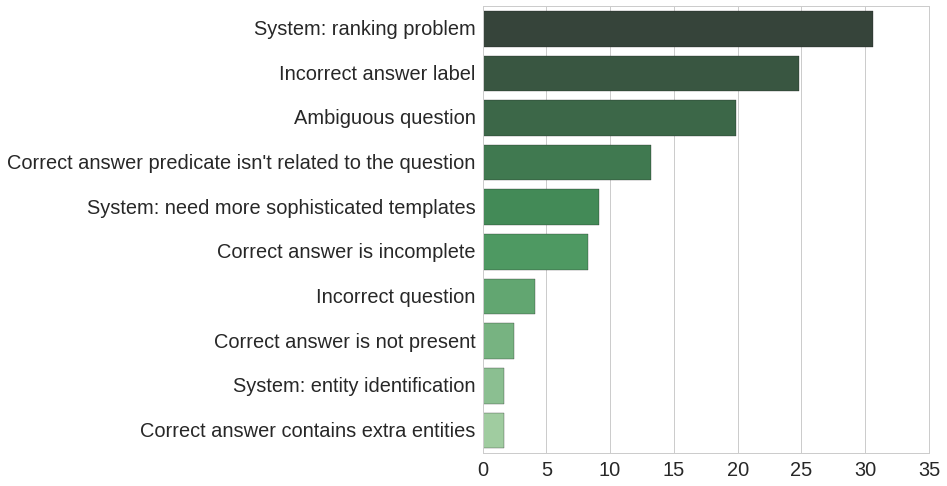
\includegraphics[width=0.45\textwidth]{img/error_analysis}
\caption{Distribution of problems with examples, where Text2KB returns an answer with F1$\neq$1.0}
\label{fig:error_analysis}
\end{figure}

To get a better insights of the problems that remain, we collected 1219 questions for which Text2KB didn't return completely correct answer, \ie F1 score of the answer is less than 1.
We manually looked through a couple of hundreds of these examples  and grouped the problems into several clusters, the results are summarized on Figure \ref{fig:error_analysis}.

As we can see candidate ranking is still the major problem, however, it accounts for $~31\%$ of the cases.
The second most popular problem is incorrect ground truth labels, which by our estimate accounted for almost a quarter of incorrect answers.
For example: for the question \textit{when tupac was shot?''} the label says \texttt{Tupac 1994 assault} instead of \texttt{Las Vegas} as the ground truth.
A related set of questions have incomplete or overcomplete set of ground truth answer entities.
A typical examples are questions asking for a list of movies, books, landmarks.
The ground truth answer usually contains $\sim10$ entities, whereas the full list is often much larger.
This seems to be an artifact of the labeling process, where the answer was selected from the Freebase entity profile page.
The profile page shows only a sample of 10 entities from large lists and the other are hidden behind the ``NNN values total'' link, which needs to be clicked in order to get the full list.
About 20\% of the questions are ambiguous, \ie questions have no strict 1-1 correspondence with any of the predicates and can be answered by multiple without any obvious preferences.
For example, for the question \textit{``where is shakira from?''} the ground truth is the country - \texttt{Colombia}, while Text2KB returned her place of birth - \texttt{Barranquilla}.
Another example are questions like \textit{``what did hayes do?''}, which can be answered by profession, occupied position or some other achievements.
Another problem is when there is no predicate that answers the question.
For example, the question \textit{``what do people in france like to do for fun?''} doesn't have a good match among the facts stored in Freebase.
The ground truth entity \texttt{Cycling} comes from predicate related to the olympic sport competitions country participated in\footnote{\texttt{olympics.olympic\_participating\_country.athletes}}, which obviously isn't related to the question.
% In some cases there are entities that are very similar in meaning, but represented in Freebase by different ids and names.
% For example, the answer to the question \textit{``what is william taft famous for?''} is \textit{``President of the United States''}, which is a government position, but there is also a triple \texttt{[William Howard Taft, common.topic.notable\_for, US President]}, where the last entity represents a type of people who help the position, and is considered incorrect.

% This is nice, but probably is too little to mention.
% We also noticed, that in a small number of examples, the case of the correct answer entity and the answer returned by the system is different.
% For example, for the question \textit{``what fma stands for?''} the correct answer specified in the dataset is \textit{``FullMetal Alchemist''}, while the actual name of the entity is \textit{``Fullmetal Alchemist''}.
% The official evaluation script don't normalize the case and therefore considers this example incorrect.
% If we lowercase all entity names before comparison, the average F1 score of Text2KB becomes 0.5248.

As for the system errors, we didn't observe any dominant problems.
There are wins and loses introduced by each of our components.
Web search results helped identify the right question topical entity in a number of cases, \eg the question \textit{``what did romo do?''} mentions only the last name of the Dallas Cowboys quarterback and the baseline system were unable to map it to the right entity.
Web search results provided more than enough evidence that romo refers to \texttt{Tomo Romo}.
However, there are a number of loses, introduced by added unrelated entities.
For example, the entity \texttt{I Love Lucy} was added for the question \textit{``what was lucille ball?''}, because the term \textit{lucy} had high similarity with \textit{lucille}.
A portion of these problems can be fixed by a better entity linking strategy, \eg \cite{SMAPH_ERD:2014}.

% For the question \textit{``what did bruce jenner win gold medal for?''} the baseline system answered \textit{``1976 Summer Olympics''}, but web search results mention decathlon many times and thus Text2KB was able to rerank the candidates and return the entity \textit{``Athletics at the 1976 Summer Olympics - Men's Decathlon''}\footnote{Unfortunately, the entity selected as the answer during labeling is \textit{``Decathlon Challenge''}, which is a book Bruce Jenner wrote}.

An interesting example, when external text resources improved the performance is the question \textit{``what ship did darwin sail around the world?''}.
This is actually a hard question, because the ship entity is connected to the \texttt{Charles Darwin} entity through the ``known for'' predicate\footnote{\texttt{user.lindenb.default\_domain.scientist.known\_for}} along with some other entities like \texttt{Natural selection}.
Thus, the predicate itself isn't related to the question, but nevertheless, the name of the ship \texttt{HMS Beagle} is mentioned multiple times in the web search results, and entity pair model computed from ClueWeb also has high scores for the terms ``ship'' and ``world''.

There are several major reasons for the loses, introduced by features based on external text resources.
Some entities often mentioned together and therefore one of such entities gets high values of cooccurrence features.
For example, the baseline system answered the question \textit{``when did tony romo got drafted?''} correctly, but since \texttt{Tony Romo} is often followed by \texttt{Dallas Cowboys}, Text2KB ranked the team name higher.
Another common problem with our features is an artifact of entity linking, which works better for names and often skips abstract entities, like professions.
For example, the correct answer to the question \textit{``what did jesse owens won?''} is an entity with the name \texttt{Associated Press Male Athlete of the Year}, which is rarely mentioned or it's hard to find such mentions.
Some problems were introduced by a combination of components.
For example, for the question \textit{``where buddha come from?''} a topical entity \texttt{Buddhism} was introduced from search results, and it generated \texttt{Gautama Buddha} as one of the answer candidates.
This answer was ranked highest due to large number of mentions in the search results.

Some errors of the original system 
Relation score is still highest importance, and missing predicates produce low score.
what country was slovakia?
It also biases everything, popular predicates like profession dominate. Also contains.

who played elaine the pain? -> search results aren't very well.

% I already mentioned this...
% WebQuestions dataset isn't free of noise and quite a few answers are actually incorrect for various reasons.
% When labeling the question ``what team does jordan own?'' mechanical turk workers had to select the answer from the page, corresponding to the country and not \textit{Michael Jordan} the basketball player.


% Non-relevant
% The first set of improvements come from the date range filter template, \eg for the question \textit{``who is the current leader of france 2010?''} our system returns a single correct result \textit{``Nicolas Sarkozy''} instead of the list of all French presidents.
% The type model score feature helped in some cases, where there is a clear indication of the type of entity, expected as the answer, \eg \textit{``which state did anne hutchinson found?''} - \textit{``Rhode Island''}.